\section{习题一}

\subsection{热身题}

\begin{problem}{1.2}{1}
  把有 \( n \) 个圆盘的塔从左边的桩柱 \( A \) 移动到右边的桩柱 \( B \)，不允许在 \( A \) 和 \( B \) 之间直接移动，求最短的移动序列。（每一次移动都必须是移动到中间的桩柱或者从中间的桩柱移出。像通常一样，较大的圆盘永远不能放在较小圆盘的上面。）
\end{problem}

将原来汉诺塔中，从 \( A \) 直接到 \( B \) 的步骤转化为以 \( C \) 作为过渡进行移动，因此，解出
\[
  T(n) = 3^n - 1
\]

下面用数学归纳法证明：
\begin{enumerate}
  \item 当 \( n=1 \) 时，将圆盘从 \( A \) 移到 \( C \) 再到 \( B \)，共花费 \( T(1) = 3^1 - 1 = 2 \) 步
  \item 假设当 \( n=k \) 时，将圆盘从 \( A \) 移到 \( B \) 需要花费 \( T(k) = 3^k - 1 \) 步
  \item 则当 \( n=k+1 \) 时，先将前 \( k \) 个圆盘移到 \( B \) 桩，花费 \( T(k) \) 步，再将第 \( k+1 \) 个圆盘移到 \( C \) 桩，花费1步；接着将前 \( k \) 个圆盘移回 \( A \) 桩，花费 \( T(k) \) 步，将第 \( k+1 \) 个圆盘移到 \( B \) 桩，花费1步；最后将 \( k \) 个圆盘再移动到 \( B \) 桩，花费 \( T(k) \) 步。因此，总共花费了 \( T(k+1) = 3T(k) + 2 \) 步，即有 \( T(k+1) = 3(3^k - 1) + 2 = 3^{k+1} - 1 \)
\end{enumerate}
\hfill \( \square \)

\begin{problem}{1.6}{1}
  平面上由 \( n \) 条直线定义的某些区域是无界的，而另一些区域则是有界的。有界区域的最大个数是多少？
\end{problem}

前面已经证出，平面上 \( n \) 条直线所界定的区域的最大个数 \( L_n = \frac{n(n+1)}{2} + 1, \ n \ge 0 \)，因此，要求有界区域的最大个数，即相当于无界区域个数最少时的情形。而经过仔细观察 \( n=3 \) 到 \( n=4 \) 时无界区域个数的变化情况，会发现在区域 1 和 2 新增加了 2 个无界区域。

\begin{center}
  \tikzset{every picture/.style={line width=0.75pt}}  % set default line width to 0.75pt
  \begin{tikzpicture}[x=0.75pt,y=0.75pt,yscale=-1,xscale=1]
    % uncomment if require: \path (0,285); %set diagram left start at 0, and has height of 285
    \path (50, 220);
    %Straight Lines [id:da19583004579399144]
    \draw    (155.4,67.5) -- (259.4,200.5) ;
    %Straight Lines [id:da007141895747585725]
    \draw    (202.87,76.44) -- (156.4,207.5) ;
    %Straight Lines [id:da6087469566187116]
    \draw    (114.4,153.5) -- (279.4,142.5) ;
    %Straight Lines [id:da0623191872932074]
    \draw    (459.4,70.5) -- (563.4,203.5) ;
    %Straight Lines [id:da7342999845570857]
    \draw    (506.87,79.44) -- (460.4,210.5) ;
    %Straight Lines [id:da2724852495866712]
    \draw    (418.4,156.5) -- (583.4,145.5) ;
    %Straight Lines [id:da705517355468706]
    \draw    (434.4,189.5) -- (558.4,112.5) ;

    % Text Node
    \draw (441,195) node [anchor=north west][inner sep=0.75pt]  [color={rgb, 255:red, 255; green, 0; blue, 0 }  ,opacity=1 ] [align=left] {1};
    % Text Node
    \draw (552,125) node [anchor=north west][inner sep=0.75pt]  [color={rgb, 255:red, 255; green, 0; blue, 0 }  ,opacity=1 ] [align=left] {2};
  \end{tikzpicture}
\end{center}

由此易得当第 \( n \) 条直线与前 \( n-1 \) 条直线相交于 \( n-1 \) 个不同点时，每次增加的无界区域最小为 \( 2n \) 个。因此，有界区域的最大个数
\begin{align*}
  T(n) = \frac{n(n+1)}{2} + 1 - 2n = \frac{1}{2}n^2 - \frac{3}{2}n + 1, \ n \ge 0
\end{align*}

\begin{problem}{1.7}{1}
  设 \( H(n) = J(n+1) - J(n). \) 方程（1.8）告诉我们有 \( H(2n) = 2 \)，而对 \( n \geq 1 \) 有
  \[
    H(2n+1) = J(2n+2) - J(2n+1) = (2J(n+1) - 1) - (2J(n) + 1) = 2H(n) - 2
  \]
  于是，看起来有可能通过对 \( n \) 用归纳法，证明对所有 \( n \) 都有 \( H(n) = 2 \)。这里什么地方有错？
\end{problem}

由 \( J \) 的定义式：
\begin{align*}
  J(1) &=1 \\
  J(2n) &= 2J(n) - 1, \ n \ge 1 \\
  J(2n+1) &= 2J(n) + 1, \ n \ge 1
\end{align*}
得：\( J(2) = 2J(1) - 1 = 1 \)，而 \( H(n) = J(n+1) - J(n) \)，所以 \( H(1) = J(2) - J(1) = 0 \ne 2 \)，因此归纳法的基础情况不满足。

\subsection{作业题}

\begin{problem}{1.8}{2}
  解递归式
  \begin{align*}
    Q_0 &= \alpha; \quad Q_1 = \beta; \\
    Q_n &= (1 + Q_{n-1}) / Q_{n-2}, \quad n > 1.
  \end{align*}
  假设对所有 \( n \geq 0 \) 都有 \( Q_n \neq 0 \)。\textit{提示：}\( Q_4 = (1 + \alpha) / \beta \).
\end{problem}

按照 \( Q_n \) 的定义式：\( Q_n = \frac{1 + Q_{n-1}}{Q_{n-2}}, \ n > 1 \)，计算下去：
\begin{align*}
  Q_0 &= \alpha \\
  Q_1 &= \beta \\
  Q_2 &= \frac{1+ \beta}{\alpha} \\
  Q_3 &= \frac{1+ \alpha + \beta}{\alpha \beta} \\
  Q_4 &= \frac{1+ \alpha}{\beta} \\
  Q_5 &= \alpha \\
  Q_6 &= \beta \\
  \dots
\end{align*}
易得，\( Q_n \) 的周期为 5，因此有：\( Q_n = Q_{n+5} \)

\begin{problem}{1.9}{2}
  有时可以利用反向归纳法，它是从 \( n \) 到 \( n-1 \) 来证明命题，而不是相反！例如，考虑命题
  \[
    P(n): \ x_1 \cdots x_n \leq \left( \frac{x_1 + \cdots + x_n}{n} \right)^n, \ x_1, \cdots, x_n \geq 0.
  \]
  这对 \( n=2 \) 为真，因为 \( (x_1 + x_2)^2 - 4 x_1 x_2 = (x_1 - x_2)^2 \geq 0 \).

  \begin{enumerate}
    \item[a] 令 \( x_n = (x_1 + \cdots + x_{n-1}) / (n-1) \)，证明只要 \( n>1 \)，\( P(n) \) 就蕴含 \( P(n-1) \).
    \item[b] 证明 \( P(n) \) 和 \( P(2) \) 蕴涵 \( P(2n) \).
    \item[c] 说明为什么这就蕴涵了 \( P(n) \) 对所有 \( n \) 为真。
  \end{enumerate}
\end{problem}

a. 若 \( P(n) \) 成立，即有
\begin{align*}
  x_1 \dots x_n &\le (\frac{x_1 + \dots + x_n}{n})^n, \ x_1, \dots, x_n \ge 0 \\
  \xrightarrow{x_n = \frac{x_1 + \dots + x_{n-1}}{n-1}} x_1 \dots x_{n-1} \frac{x_1 + \dots + x_{n-1}}{n-1} &\le (\frac{x_1 + \dots + x_{n-1} + \frac{x_1 + \dots + x_{n-1}}{n-1}}{n})^n \\
  \Leftrightarrow x_1 \dots x_{n-1} \frac{x_1 + \dots + x_{n-1}}{n-1} &\le (\frac{x_1 + \dots + x_{n-1}}{n-1})^n \\
  \Leftrightarrow x_1 \dots x_{n-1} &\le (\frac{x_1 + \dots + x_{n-1}}{n-1})^{n-1}
\end{align*}
所以，对于 \( P(n-1) \) 也成立。

b. 若 \( P(2) \) 和 \( P(n) \) 成立，有：
\begin{align*}
  P(n): \ x_1 \dots x_n &\le (\frac{x_1 + \dots + x_n}{n})^n \\
  P'(n): \ x_{n+1} \dots x_{2n} &\le (\frac{x_{n+1} + \dots + x_{2n}}{n})^n
\end{align*}
所以：
\begin{equation*}
  (x_1 \dots x_n)(x_{n+1} \dots x_{2n}) \le (\frac{(x_1 + \dots + x_n)(x_{n+1} + \dots + x_{2n})}{n^2})^n
\end{equation*}
又：
\begin{align*}
  P(2): \ x_1 x_2 &\le (\frac{x_1 + x_2}{2})^2 \\
  \Rightarrow (x_1 + \dots + x_n)(x_{n+1} + \dots + x_{2n}) &\le (\frac{x_1 + \dots + x_{2n}}{2})^2
\end{align*}
所以：
\begin{equation*}
  x_1 \dots x_n x_{n+1} \dots x_{2n} \le(\frac{(\frac{x_1 + \dots + x_{2n}}{2})^2}{n^2})^n =(\frac{x_1 + \dots + x_{2n}}{2n})^{2n}
\end{equation*}
即证 \( P(2n) \) 也成立。

c. 由 a,b 易知：
\begin{align*}
  &P(2) \rightarrow P(1); \\
  &P(2) \wedge P(2) \rightarrow P(4) \rightarrow P(3) \rightarrow P(6) \rightarrow P(5) \rightarrow \dots
\end{align*}
所以 \( P(n) \) 对所有 \( n \) 为真。

\begin{problem}{1.10}{2}
  设 \( Q_n \) 是将一个有 \( n \) 个圆盘的塔从 \( A \) 移动到 \( B \) 所需要的最少移动次数，要求所有的移动都必须是顺时针方向的，也就是说，从 \( A \) 到 \( B \)，从 \( B \) 到其他的桩柱，再从其他的桩柱到A。又设 \( R_n \) 是在这一限制下从 \( B \) 返回到 \( A \) 所需要移动的最少次数。证明
  \[
    Q_n =
    \begin{cases}
      0, & n = 0; \\
      2R_{n-1} + 1, & n > 0;
    \end{cases} \quad
    R_n =
    \begin{cases}
      0, & n = 0; \\
      Q_n + Q_{n-1} + 1, & n > 0.
    \end{cases}
  \]
  （无需解这些递归式，我们将在第 7 章里介绍怎样做。）
\end{problem}

如图：
\begin{center}
  \tikzset{every picture/.style={line width=0.75pt}} %set default line width to 0.75pt
  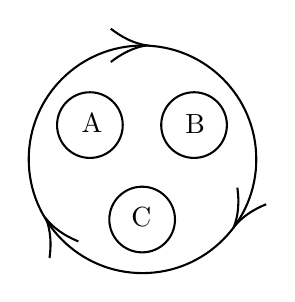
\begin{tikzpicture}[x=0.75pt,y=0.75pt,yscale=-1,xscale=1]
    %Shape: Circle [id:dp9551136057365387]
    \draw   (292.67,136.01) .. controls (292.67,105.74) and (317.21,81.19) .. (347.49,81.19) .. controls (377.76,81.19) and (402.31,105.74) .. (402.31,136.01) .. controls (402.31,166.29) and (377.76,190.83) .. (347.49,190.83) .. controls (317.21,190.83) and (292.67,166.29) .. (292.67,136.01) -- cycle ;
    %Shape: Circle [id:dp7600036702259039]
    \draw   (306.33,119.51) .. controls (306.33,110.78) and (313.42,103.69) .. (322.15,103.69) .. controls (330.89,103.69) and (337.97,110.78) .. (337.97,119.51) .. controls (337.97,128.25) and (330.89,135.33) .. (322.15,135.33) .. controls (313.42,135.33) and (306.33,128.25) .. (306.33,119.51) -- cycle ;
    %Shape: Circle [id:dp2475680419776638]
    \draw   (356.5,119.51) .. controls (356.5,110.78) and (363.58,103.69) .. (372.32,103.69) .. controls (381.06,103.69) and (388.14,110.78) .. (388.14,119.51) .. controls (388.14,128.25) and (381.06,135.33) .. (372.32,135.33) .. controls (363.58,135.33) and (356.5,128.25) .. (356.5,119.51) -- cycle ;
    %Shape: Circle [id:dp07583722775456803]
    \draw   (331.5,165.01) .. controls (331.5,156.28) and (338.58,149.19) .. (347.32,149.19) .. controls (356.06,149.19) and (363.14,156.28) .. (363.14,165.01) .. controls (363.14,173.75) and (356.06,180.83) .. (347.32,180.83) .. controls (338.58,180.83) and (331.5,173.75) .. (331.5,165.01) -- cycle ;
    \draw   (332.22,73.08) .. controls (337.96,77.54) and (343.7,80.21) .. (349.44,81.1) .. controls (343.7,81.99) and (337.96,84.66) .. (332.22,89.11) ;
    \draw   (407.08,157.65) .. controls (400.35,160.39) and (395.17,164.02) .. (391.53,168.55) .. controls (393.63,163.13) and (394.18,156.83) .. (393.2,149.63) ;
    \draw   (302.7,183.56) .. controls (303.69,176.36) and (303.13,170.06) .. (301.03,164.64) .. controls (304.67,169.17) and (309.86,172.8) .. (316.58,175.55) ;

    % Text Node
    \draw (316.67,112.33) node [anchor=north west][inner sep=0.75pt]   [align=left] {A};
    % Text Node
    \draw (366.67,112.83) node [anchor=north west][inner sep=0.75pt]   [align=left] {B};
    % Text Node
    \draw (340.67,157.83) node [anchor=north west][inner sep=0.75pt]   [align=left] {C};
  \end{tikzpicture}
\end{center}

\( Q_n \) 代表按顺时针将 \( n \) 个圆盘从 \( A \) 移到 \( B \) 的最少移动次数，\( R_n \) 代表按顺时针将 \( n \) 个圆盘从 \( B \) 返回 \( A \) 的最少移动次数。理解的关键在于观察到 \( Q_n \) 需要移动的两个桩柱是相邻的，而 \( R_n \) 需要移动的桩柱之间隔了一根。
因此：
\begin{equation*}
  Q_n =
  \begin{cases} 0 & n = 0, \\
    2R_{n-1} + 1 & n > 0, \\
  \end{cases}
\end{equation*}
意即先将前 \( n-1 \) 个圆盘从 \( A \) 移到 \( C \)，花费 \( R_{n-1} \) 步；再将第 \( n \) 个圆盘移到 \( B \)，花费1步；最后再将 \( n-1 \) 个圆盘从 \( C \) 移到 \( B \)，花费 \( R_{n-1} \) 步。
\begin{equation*}
  R_n=
  \begin{cases} 0 & n = 0, \\
    2R_{n-1} + 1 + Q_{n-1} + 1 = Q_n + Q_{n-1} + 1 & n > 0, \\
  \end{cases}
\end{equation*}
意即先将前 \( n-1 \) 个圆盘从 \( B \) 移到 \( A \)，花费 \( R_{n-1} \) 步；再将第 \( n \) 个圆盘从 \( B \) 移到 \( C \)，花费1步；再将前 \( n-1 \) 个圆盘从 \( A \) 移到 \( B \)，花费 \( Q_{n-1} \) 步；接着将第 \( n \) 个圆盘从 \( C \) 移到 \( A \)，花费1步；最后将前 \( n-1 \) 个圆盘从 \( B \) 移到 \( A \)，花费 \( R_{n-1} \) 步。

\begin{problem}{1.11}{2}
  双重河内塔包含 \( 2n \) 个圆盘,它们有 \( n \) 个不同的尺寸，每一种尺寸的圆盘有两个。如通常那样，要求每次只能移动一个圆盘，且不能把较大的圆盘放在较小的圆盘上面。

  \begin{enumerate}
    \item[a] 如果相同尺寸的圆盘是相互不可区分的，要把一个双重塔从一根桩柱移动到另一根桩柱需要移动多少次？
    \item[b] 如果在最后的排列中要把所有同样尺寸的圆盘恢复成原来的从上到下的次序，需要移动多少次？\textit{提示：}这是一个难题，实在应该是个“附加题”。
  \end{enumerate}
\end{problem}

a. 因为相同尺寸的圆盘是不可区分的，且每一种尺寸的圆盘有两个。记有 \( n \) 种不同的圆盘，易得：
\begin{align*}
  A_1 &= 2 \\
  A_n &= 2 A_{n-1} + 2, \ n > 1
\end{align*}
再算出它的封闭形式：
\begin{align*}
  A_n + 2 &= 2(A_{n-1} + 2) \\
  \xrightarrow{C_n = A_n + 2} C_n &= 2 C_{n-1} \\
  \Rightarrow C_n &= 2^{n+1} \\
  \Rightarrow A_n &= 2^{n+1} - 2
\end{align*}

b. 如果需要在最后的排列中将所有同样尺寸的圆盘恢复到原来的上下顺序，则对于 \( n \) 种圆盘（\( 2n \) 个圆盘），有：
\begin{align*}
  B_1 &= 3 \\
  B_n &= A_{n-1} + 2 + A_{n-1} + 2 + B_{n-1}, \ n>1
\end{align*}
假设是将 \( n \) 种圆盘（每种两个）从 \( A \) 柱移到 \( B \) 柱，以 \( C \) 柱为过渡。先将前 \( n-1 \) 种圆盘不计顺序的从 \( A \) 移到 \( B \)，花费 \( A_{n-1} \) 步；再将最后1种圆盘从 \( A \) 移到 \( C \)，此时这2个圆盘在 \( C \) 柱上的顺序应该是反向的，花费2步；接着将前 \( n-1 \) 种圆盘不计顺序的从 \( B \) 回到 \( A \)，花费 \( A_{n-1} \) 步；此时将 \( C \) 柱上的两个反向的圆盘移到 \( B \) 柱上，这样两个圆盘就可以按照正确的顺序落在 \( B \) 柱上，花费 2 步；最后将前 \( n-1 \) 种圆盘按顺序的从 \( A \) 移到 \( B \)，花费 \( B_{n-1} \) 步

再算出它的封闭形式：
\begin{align*}
  B_n & = 2 (2^n - 2) + 4 + B_{n-1} \\
  \Rightarrow B_n &= B_{n-1} + 2^{n+1} \\
  \Rightarrow B_2 &= B_1 + 2^3 \\
  B_3 &= B_2 + 2^4 \\
  B_4 &= B_3 + 2^5 \\
  \vdots
  \\ B_n &= B_{n-1} + 2^{n+1} \\
  \Rightarrow S_n - B_1 &= S_{n-1} + \frac{2^3(2^{n-1} - 1)}{2 - 1} \\
  \Rightarrow S_n - S_{n-1} = B_n &= 2^{n+2} - 5
\end{align*}

\begin{problem}{1.13}{2}
  由 \( n \) 条 \( Z \) 形线所定义的区域的最大个数是多少？每条 \( Z \) 形线由两条平行的无限半直线和一条直线段组成。
\end{problem}

我们可以将眼前的直线看作是有着极其细微的 \( Z \) 型折痕：

\begin{center}
  \tikzset{every picture/.style={line width=0.75pt}} %set default line width to 0.75pt
  \begin{tikzpicture}[x=0.75pt,y=0.75pt,yscale=-1,xscale=1]
    %uncomment if require: \path (0,286); %set diagram left start at 0, and has height of 286
    \path(50, 240);
    %Straight Lines [id:da02812046425774839]
    \draw    (460.4,50.7) -- (621.4,222.7) ;
    %Straight Lines [id:da47182775430134694]
    \draw    (600.4,56.7) -- (460.4,206.7) ;
    %Straight Lines [id:da3215292568144861]
    \draw    (88.4,47.7) -- (184.2,143.5) ;
    %Straight Lines [id:da3245507540140673]
    \draw    (228.4,53.7) -- (136.7,145.4) ;
    %Straight Lines [id:da9234938262765493]
    \draw    (182.25,124.85) -- (86.4,220.7) ;
    %Straight Lines [id:da8106487734605339]
    \draw    (136.7,123) -- (257.4,243.7) ;
    %Straight Lines [id:da2007154674512137]
    \draw    (136.7,145.4) -- (182.25,124.85) ;
    %Straight Lines [id:da7448969942232411]
    \draw    (136.7,123) -- (184.2,143.5) ;
  \end{tikzpicture}
\end{center}

因此，可以仿照直线切割平面区域来思考。同时又观察到，原本的每个交点现在会多增加 8 个区域，所以列出下面的递推方程：
\begin{align*}
  Z_1 &= 2 \\
  Z_n &= Z_{n-1} + n + 8(n-1), \ n>1
\end{align*}
意即，当第 \( n \) 条直线在 \( n-1 \) 个不同地方与前面那些直线相交，会使区域个数新增加 \( n \) 个（这是直线切割的情况），再加上 Z 型交点新增加的 \( 8(n-1) \) 个区域。进而算出它的封闭形式：
\begin{align*}
  Z_2 &= Z_1 + 9*2 - 8 \\
  Z_3 &= Z_2 + 9*3 - 8 \\
  \vdots \\
  Z_n &= Z_{n-1} + 9n - 8 \\
  \Rightarrow S_n - 2 &= S_{n-1} + 9(\frac{(n-1)(2+n)}{2}) - 8(n-1) \\
  \Rightarrow S_n - S_{n-1} = Z_n &= \frac{9}{2} n^2 - \frac{7}{2} n + 1
\end{align*}

\begin{problem}{1.14}{2}
  在一块厚奶酪上划出五道直的切痕，可以得到多少块奶酪？（在你划切痕时，奶酪必须保持在它原来的位置上，且每道切痕必定与三维空间中的一个平面相对应。）对 \( P_n \) 求一个递归关系，这里 \( P_n \) 表示 \( n \) 个不同的平面所能定义的三维区域的最大个数。
\end{problem}

首先计算出 \( n \) 很小时，\( P_n \) 的值：
\begin{align*}
  P_1 &= 2 \\
  P_2 &= 4 \\
  P_3 &= 8
\end{align*}
也许看上去很像是 \( P_n = 2^n \) 的关系，但实际上这是不可能的，因为不能保证每一刀都能触碰到之前分出的每一块。而要想让第 \( n \) 刀切下去时，蛋糕尽量分出更多份，需要保证前面 \( n-1 \) 个切痕在这第 \( n \) 刀形成的平面上分出尽量多的区域，问题即转化为平面的直线分割。因此，\( P_n \) 的递推公式为：\( P_n = P_{n-1} + L_{n-1} \)

\begin{problem}{1.15}{2}
  约瑟夫有一个朋友，他站在倒数第二的位置上因而获救。当每隔一个人就有一人被处死时，倒数第二个幸存者的号码 \( I(n) \) 是多少？
\end{problem}

要计算约瑟夫环的倒数第二个幸存者 \( I(n) \) 的号码，首先考虑基础情况：当 \( n \) 为 2 时，易知 \( I(2) = 2 \)，接着可以先算出 \( n \) 比较小时的情况，以此来观察规律：

\begin{table}[ht]
  \centering
  \arrayrulecolor{grayblack}
  \rowcolors{1}{white}{gray}
  {\color{grayblack}
    \begin{tabular}{p{4cm}cc}
      \toprule
      \rowcolor{bluegray}
      \( \mathbf{n} \)  & \( \mathbf{I(n)} \) \\
      \midrule
      2 & 2 \\
      3 4 5 & 1 3 5 \\
      6 7 8 9 10 11 & 1 3 5 7 9 11 \\
      12 \( \dots \) & 1 \( \dots \) \\
      \( \dots \) & \( \dots \) \\
      \bottomrule
  \end{tabular}}
\end{table}

写到这份上时，就很明显了，有：
\begin{align*}
  I(2) &= 2 \\
  I(3 * 2^m + l) &= 2l + 1, \ m \ge 0, \ 0 \le l < 2^m
\end{align*}

\begin{problem}{1.16}{2}
  用成套方法来求解一般的四参数递归式
  \begin{align*}
    g(1) &= \alpha; \\
    g(2n + j) &= 3g(n) + \gamma n + \beta_j; \quad j = 0, 1, \ n \geq 1
  \end{align*}
  \textit{提示：}尝试用函数 \( g(n) = n \).
\end{problem}

首先看一种递归式的有趣的解法：
\begin{align*}
  f(1) &= \alpha \\
  f(2n + j) &= 2f(n) + \beta_{j} \quad j = 0, 1 \quad n \ge 1
\end{align*}
将它按照二进制展开：
\begin{align*}
  f((b_m b_{m-1} \dots b_1 b_0)_2) &= 2f((b_m b_{m-1} \dots b_1)_2) + \beta_{b_0} \\
  &= 4f((b_m b_{m-1} \dots b_2)_2) + 2 \beta_{b_1} + \beta_{b_0} \\
  &\vdots \\
  &= 2^{m}f((b_m)_2) + 2^{m-1} \beta_{b_{m-1}} + \dots + 2 \beta_{b_1} + \beta_{b_0} \\
  &= 2^m \alpha + 2^{m-1} \beta_{b_{m-1}} + \dots + 2 \beta_{b_1} + \beta_{b_0}
\end{align*}
解除二进制的表示，从而允许各位上是任意数字，则有：
\begin{equation*}
  f((b_m b_{m-1} \dots b_1 b_0)_2 ) = (\alpha \beta_{b_{m-1}} \beta_{b_{m-2}} \dots \beta_{b_1} \beta_{b_0})_2
\end{equation*}
再进一步推广，又有：
\begin{align*}
  f(j) &= \alpha_j \quad 1 \le j < d \\
  f(dn + j) &= cf(n) + \beta_j \quad 0 \le j < d, \ n \ge 1 \\
  \Rightarrow f((b_m b_{m-1} \dots b_1 b_0)_d) &= (\alpha_{b_m} \beta_{b_{m-1}} \beta_{b_{m-2}} \dots \beta_{b_1} \beta_{b_0})_c
\end{align*}
这里从基数为 \( d \) 的数开始，结果表示为基数为 \( c \) 的数。

而这道题目：
\begin{align*}
  g(1) &= \alpha \\
  g(2n+j) &= 3g(n) + \gamma n + \beta_j \quad j = 0, 1 \quad n \ge 0
\end{align*}
首先设：\( g(n) = a(n) \alpha + b(n) \beta_0 + c(n) \beta_1 + d(n) \gamma \)，当 \( n= (b_m b_{m-1} \dots b_1 b_0)_2 \quad (b_m \ne 0) \)，按照上面的思路，有：
\begin{align*}
  &\phantom{=} g(\ (b_m b_{m-1} \dots b_1 b_0)_2 \ ) \\
  &= 3g(\ (b_m b_{m-1} \dots b_1)_2 \ ) + \gamma * (b_m b_{m-1} \dots b_1)_2 + \beta_{b_0} \\
  &= 3^2g(\ (b_m b_{m-1} \dots b_2)_2 \ ) + 3 * \gamma * (b_m b_{m-1} \dots b_2)_2 + 3 \beta_{b_1} + \gamma * (b_m b_{m-1} \dots b_1)_2 + \beta_{b_0} \\
  &\phantom{=} \vdots \\
  &= (\alpha_{b_m} \beta_{b_{m-1}} \beta_{b_{m-2}} \dots \beta_{b_1} \beta_{b_0})_3 + \gamma * (0 \ (b_m)_3 \ (b_m b_{m-1})_3 \dots \ (b_m \dots b_1)_3)_3  \\
  &= a(n) \alpha + b(n) \beta_0 + c(n) \beta_1 + d(n) \gamma
\end{align*}
因此，有：
\begin{align*}
  d(n) &= (0 \ (b_m)_3 \ (b_m b_{m-1})_3 \dots \ (b_m \dots b_1)_3)_3 \\
  a(n) \alpha + b(n) \beta_0 + c(n) \beta_1 &= (\alpha_{b_m} \beta_{b_{m-1}} \beta_{b_{m-2}} \dots \beta_{b_1} \beta_{b_0})_3
\end{align*}

之后再来用成套方法（repertoire method）解决这题：

取 \( g(n) = n \)，则计算可知：\( a(n) + c(n) - d(n) = n \)；

取 \( g(n) = 1 \)，有 \( a(n) - 2b(n) - 2c(n) = 1 \)

所以：\( b(n) = \frac{a(n) - 2c(n) - 1}{2}, \quad d(n) = a(n) + c(n) - n \)

\subsection{考试题}

\begin{problem}{1.20}{3}
  利用成套方法来解一般的五参数递归式
  \begin{align*}
    h(1) &= \alpha \\
    h(2n+j) &= 4h(n) + \gamma_j n + \beta_j \quad j = 0, 1 \quad n \ge 1
  \end{align*}
  \textit{提示：}尝试用函数 \( h(n) = n \) 和 \( h(n) = n^2 \).
\end{problem}

思路和上一题一样：设 \( h(n) = a(n) \alpha + b(n) \beta_0 + c(n) \beta_1 + d(n) \gamma_0 + e(n) \gamma_1 \)，当 \( n = (1 b_{m-1} \dots b_1 b_0)_2 \) 时，有 \( a(n) \alpha + b(n) \beta_0 + c(n) \beta_1 = (\alpha \beta_{b_{m-1}} \beta_{b_{m-2}} \dots \beta_{b_0})_4 \)

若 \( h(n) = n \)，则 \( a(n)+c(n)-2d(n)-2e(n)=n \)；

若 \( h(n) = n^2 \)，则 \( a(n)+c(n)+4e(n)=n^2 \)

所以：\( d(n) = \frac{3a(n) + 3c(n) - n^2 - 2n}{4}, \ e(n) = \frac{n^2 - a(n) - c(n)}{4} \)
